\section{Introducción }

\begin{frame}{Introducción}
	\begin{columns}
		\column{.4\textwidth}
        \begin{itemize}
        \item Los incendios forestales son un problema a nivel mundial y afectan significativamente al ecosistema y a la comunidad. 

        \end{itemize}
        
        \column{.6\textwidth}
	\begin{figure}[H]
	\centering
 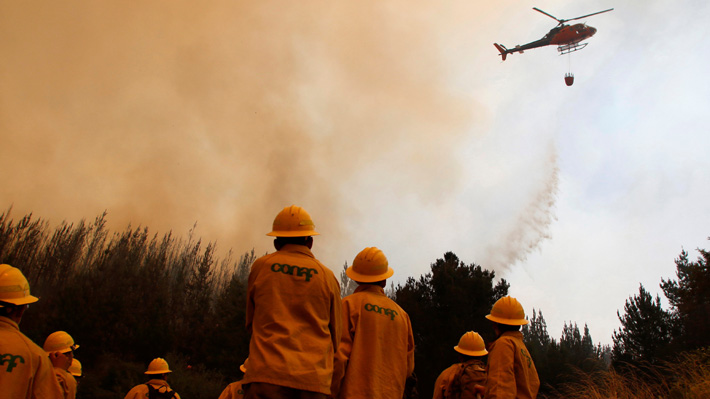
\includegraphics[width=1\textwidth]{fig/conaf.jpg}
	\end{figure}
	\end{columns}
\end{frame}




\begin{frame}{Introducción}
\centering
 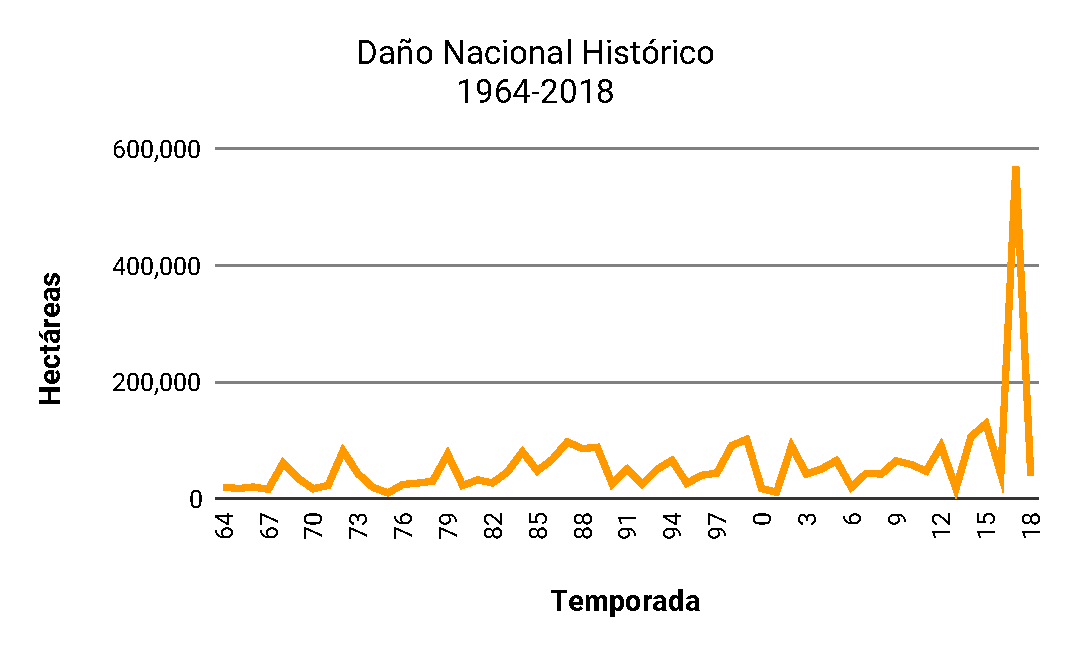
\includegraphics[width=0.8\textwidth]{fig/chart.pdf}
 \newline
 \begin{text}
En Chile, la superficie afectada por incendios forestales promedia las 57.000 hectáreas quemadas. 
\end{text}
\end{frame}











\begin{frame}{Wild Fire Watch}
	\begin{columns}
	
		\column{.4\textwidth}
        \begin{itemize}
        \item Monitoreo incendios a través de un sistema basado en drones. 
        \end{itemize}
        
        \column{.6\textwidth}
	\begin{figure}[H]
	\centering

        %
\includegraphics[width=0.1\textwidth]{fig/WFW.png}
        
 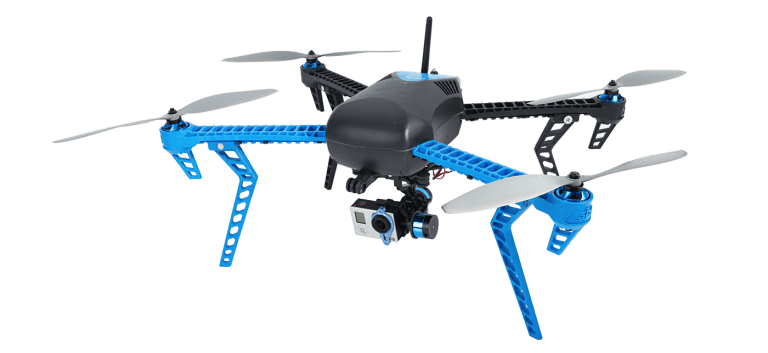
\includegraphics[width=1\textwidth]{fig/iris.png}
	\end{figure}
	\end{columns}
\end{frame}



\begin{frame}{Modelo de segmentación de fuego y humo}

	\centering
 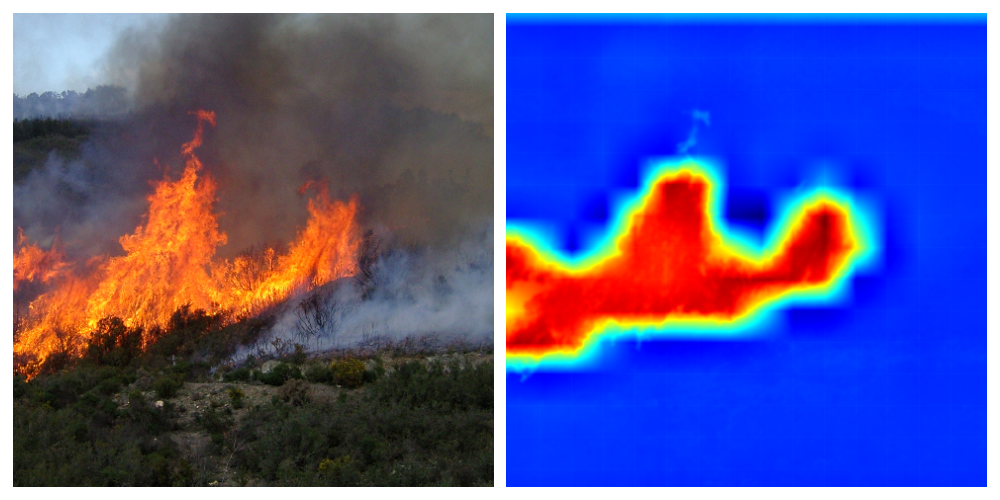
\includegraphics[width=0.5\textwidth]{fig/inferencepic.png}

Wild Fire Watch 
\end{frame}



\begin{frame}{Objetivos}
\begin{itemize}
    \item Reproducción y verificación de SFEwAN. 
    \item Análisis de tiempos. 
    \item Análisis de consumo de energía en plataformas embebidas. 
\end{itemize}
    
\end{frame}

%https://www.terram.cl/2017/03/megaincendio-de-chile-el-mas-intenso-de-la-historia/